\documentclass{article}
\usepackage[margin=1in]{geometry}
\usepackage{graphicx}
\usepackage{xcolor}
\usepackage{float}
\usepackage{amsmath}
\usepackage{cite}
\usepackage{hyperref}
\usepackage{indentfirst}
\graphicspath{{..} {./images}}

\definecolor{navy-blue}{rgb}{0.22,0.38,0.71}

\renewcommand{\contentsname}{\vspace*{-2\baselineskip}}

\hypersetup{
	colorlinks,
	linkcolor=black,
	urlcolor=blue,
	citecolor=black
}
  		
\begin{document}
\begin{titlepage}
	\centering
	{\huge Lab 6 - Digital Modulation: Carrier Synchronization}\\[0.25 in]
	
\includegraphics[width=0.6\textwidth]{ua_logo.png}\\[0.25 in]
	{\large \textbf{ECE 531 - Software Defined Radio\\[0.25 in]
	April 11, 2025\\[0.25 in]}}
	{\large Owen Sowatzke, osowatzke@arizona.edu\\[0.05 in]
	Department of Electrical \& Computer Engineering\\[0.05 in]
	University of Arizona, Tucson, AZ 85721\\[0.5 in]}
	\hypersetup{linkcolor=navy-blue}
	\noindent\hrulefill
	\tableofcontents
	\noindent\hrulefill
\end{titlepage}

% \setlength{\parindent}{0pt}

\section{Introduction}
%Introduction to the laboratory experiment, including a brief description of the objectives and goals.

\section{Procedure}
% Detailed explanation of the laboratory experiment, including the design, implementation, and testing of the system.

\section{Results}
% Results and discussion of the laboratory experiment, including captured outputs, observations, and responses to laboratory questions.

\subsection{System and Error Models}

In discrete time, when we multiply a signal by a complex exponential, it circular shifts the frequency response. If we have enough excess bandwidth, we can ensure that the significant portions of our frequency response do not wrap and in turn correctly model an analog frequency shift. If we change the `filterUpsample' in \texttt{lab6part1.m} to 1, we do have any excess bandwidth. The spectrum after a frequency shift of $0.1F_s$ is shown in Figure \ref{fig::psd_upsample_1}.

\begin{figure}[H]
	\centerline{\fbox{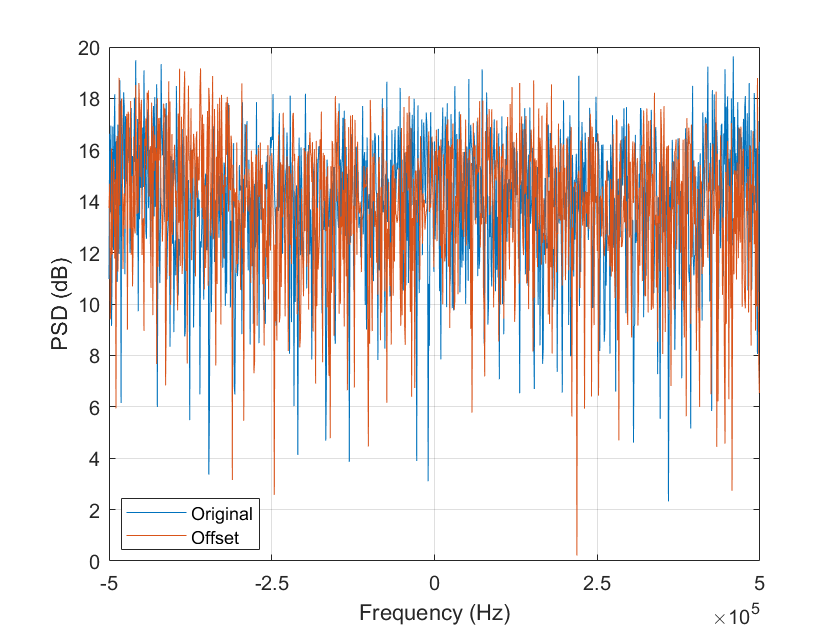
\includegraphics[width=0.5\textwidth]{psd_upsample_1.png}}}
	\caption{Frequency Response with `filterUpsample' Set to 1 and a $\protect{0.1F_s}$ Frequency Shift}
	\label{fig::psd_upsample_1}
\end{figure}

\noindent Examining the frequency response, we see that it does not correctly model a $0.1F_s$ analog frequency shift, which would have resulted in part of the spectrum being zero. Note that our updated frequency response is also not exactly a shift of the original DFT samples. This is because the DFT is sampling the DTFT. With a frequency shift of $0.1F_s$, our updated sampling positions do not overlap with the original sampling positions, which results in a slightly different response. If we instead chose a frequency shift of $F_s/16$, our sampling positions align and our DFT's are related by a simple shift. These results are captured in Figure \ref{fig::psd_upsample_1_mod_shift}.

\begin{figure}[H]
	\centerline{\fbox{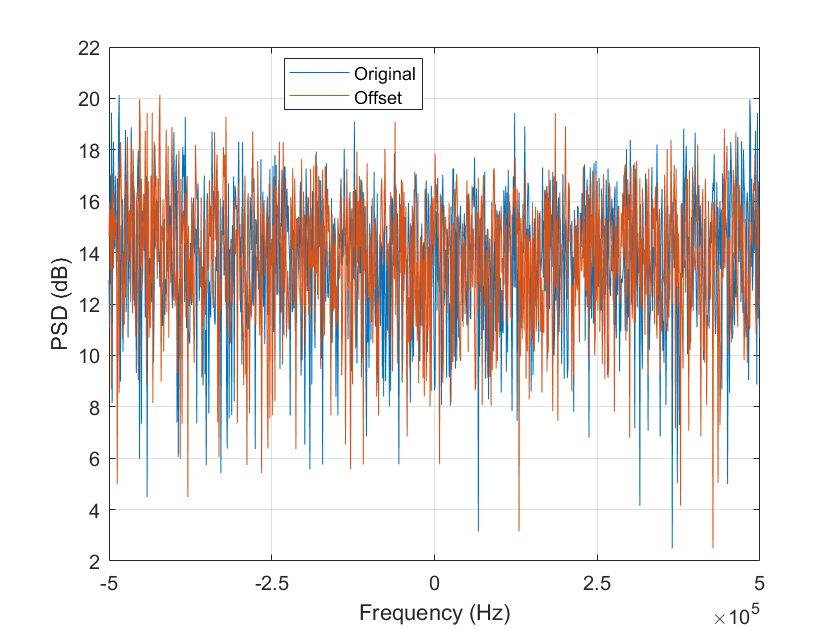
\includegraphics[width=0.5\textwidth]{psd_upsample_1_mod_shift.png}}}
	\caption{Frequency Response with `filterUpsample' Set to 1 and a $\protect{F_s/16}$ Frequency Shift}
	\label{fig::psd_upsample_1_mod_shift}
\end{figure}

\noindent We also observe a similar effect when we step the frequency offset in steps of $0.1F_s$ from $0.1F_s$ to $1.0F_s$. As we increase the frequency offset, we see the frequency response wraps. In Figure \ref{fig::psd_freq_offset_05}, we specifically show the frequency response with a frequency offset of $0.5F_s$. 

\begin{figure}[H]
	\centerline{\fbox{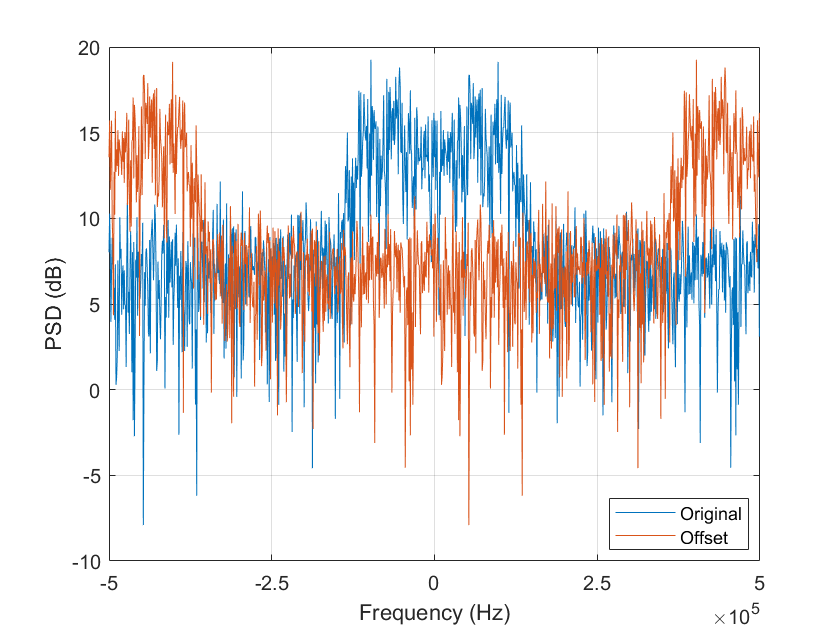
\includegraphics[width=0.5\textwidth]{psd_freq_offset_05.png}}}
	\caption{Frequency Response with a $\protect{0.5F_s}$ Frequency Shift}
	\label{fig::psd_freq_offset_05}
\end{figure}

\noindent At this frequency offset, we see that the frequency response is circularly shifted by half the bandwidth of the signal. We can explain this with DTFT properties. However, we can equivalently treat this case as an analog frequency shift prior to decimation. This results in aliasing, which in turns causes our frequency response to wrap.

	In simulation, we also increment the timing vector for each frame (\texttt{timeIndex = (k:k+frameSize-1).'}). This models back-to-back frames being fed into a continuous oscillator. The frequency offsets we observe are primarily caused by LO mismatches. However, another cause of the frequency offset is a doppler shift (which is caused by relative motion of the receiver with respect to the transmitter).

\subsection{Coarse Frequency Correction}

In this section, we perform coarse frequency correction using an FFT. To remove the modulation from our constellation, we raise our received data up to a power equivalent to the modulation order. The maximum FFT bin then gives us an index that is proportional to our estimated carrier offset. For DBPSK, the estimated carrier offset is specifically given by

\begin{equation}
	\hat{f}_0 = \frac{1}{2TK}\underset{f}{\text{argmax}}\left\vert\sum_{k=0}^{K-1}{r^2(k)e^{-j2{\pi}kT/K}}\right\vert
\end{equation}
	
\noindent When we apply coarse frequency compensation to a DBPSK-modulation signal with a $0.1F_s$ frequency offset, we obtain the spectrum shown in Figure \ref{fig::psd_bpsk_with_cfc}.

\begin{figure}[H]
	\centerline{\fbox{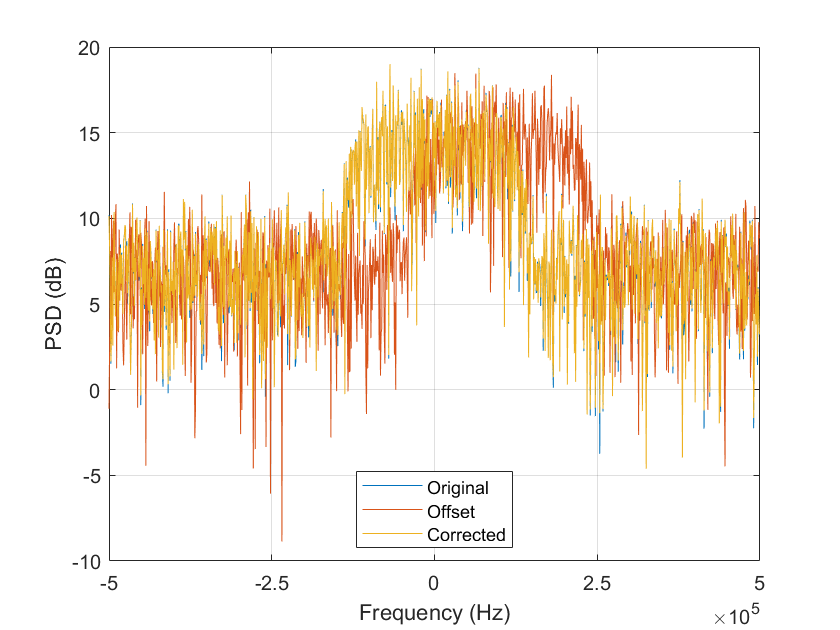
\includegraphics[width=0.5\textwidth]{psd_bpsk_with_cfc.png}}}
	\caption{DPSK Frequency Response Before and After Coarse Frequency Correction}
	\label{fig::psd_bpsk_with_cfc}
\end{figure}

\noindent Examining the figure, we see that coarse frequency correction effectively removes the carrier offset. Our spectrum before and after compensation is essentially the same.

\section{Conclusion}
% Conclusions to the overall lab that discuss meaningful lessons learned and other takeaways from the assignment. (Important)

\end{document}